\documentclass[a4paper,11pt,twocolumn]{article}

\usepackage{lrec2012}

\usepackage{polyglossia}
\setdefaultlanguage[variant=australian]{english}

\usepackage{fontspec}
\usepackage{xunicode}
\usepackage{xltxtra}
\usepackage{natbib}
\usepackage{multirow}
%\usepackage{fullpage}
\usepackage{multirow}
\usepackage[colorlinks=true,citecolor=black,linkcolor=black,urlcolor=blue]{hyperref}

\usepackage{booktabs}
\usepackage{jnwmaps}

\defaultfontfeatures{Mapping=tex-text}
\setromanfont{Times New Roman}
\newfontfamily\symbl[Scale=MatchLowercase]{FreeSerif}


\bibdata{kipchak-paper}


\title{Finite-state morphological transducers for three Kypchak languages}

\author{Jonathan North Washington \\
Departments of Linguistics and Central Eurasian Studies\\
Indiana University\\
Bloomington, IN 47405 (USA)\\
\texttt{jonwashi@indiana.edu} \and
Ilnar Salimzyanov  \\
Institut für Maschinelle Sprachverarbeitung \\
Universität Stuttgart\\
Stuttgart (Germany) \\
\texttt{ilnar@ilnar} \and 
Francis M. Tyers\\
Departament de Llenguatges i Sistemes Informàtics \\  
Universitat d'Alacant\\
E-03071 Alacant (Spain)\\
\texttt{ftyers@dlsi.ua.es} 
}

%FIXME: usually star comes first, then daggers
\name{Jonathan North Washington$^\dagger$, Ilnar Salimzyanov$^\ddagger$, Francis M. Tyers$^\star$}

\address{$^\dagger$Departments of Linguistics and Central Eurasian Studies\\
Indiana University\\
Bloomington, IN 47405 (USA)\\
\texttt{jonwashi@indiana.edu} \and
$^\ddagger$Institut für Maschinelle Sprachverarbeitung \\
Universität Stuttgart\\
Stuttgart (Germany) \\
\texttt{ilnar@ilnar} \and 
$^\star$Departament de Llenguatges i Sistemes Informàtics \\  
Universitat d'Alacant\\
E-03071 Alacant (Spain)\\
\texttt{ftyers@dlsi.ua.es} 
}

\abstract{Hargle, bargle.\\
	\Keywords{Kazakh, Tatar, Kumyk, morphology, transducer}
}

\begin{document}

\maketitleabstract{}

\section{Introduction}

This paper describes the development of morphological transducers for three closly related languages: Kazakh, Tatar, and Kumyk.


\cite{bekmanova2013}

%FIXME: brief background on how, when, and with what support were developed?
The transducers for these languages 

\section{Languages}

The three languages for which transducers were developed belong to the Northwestern branch of Turkic, which is often referred to as the Kypchak branch.  This branch can be divided into three subbranches.  Kumyk is a member of the Western Kypchak group, Tatar is a member of the Northern Kypchak group, and Kazakh is a member of the Southern Kypchak group \citep[82-83]{histofturkic}.  As such, each of these three languages represents a different one of the three branches of Kypchak.  The geographic distribution of the languages is shown in map \ref{map1}.

\begin{map*}[htbp]
	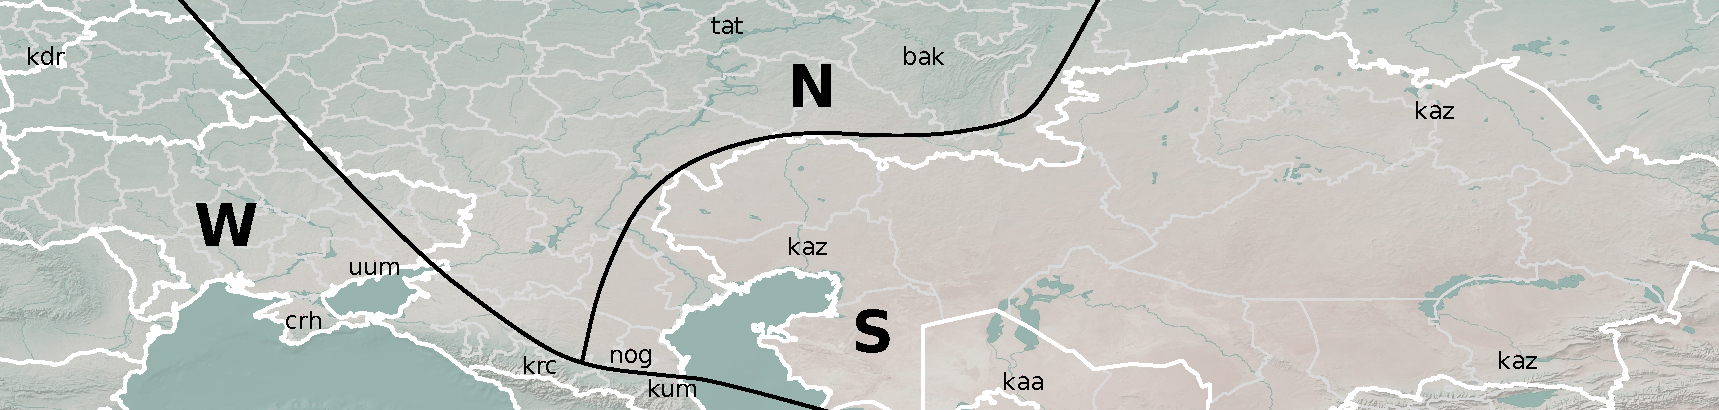
\includegraphics[width=\textwidth]{map/map}
	\caption{The three branches of Kypchak (N, S, W), showing the distribution of the three languages for which transducers were developed (tat, kaz, kum).  Language codes are from ISO 639-3.}
	\label{map1}
\end{map*}

These languages have different amounts of linguistic influence from other Turkic branches (e.g., moderate Oghuz (SE) influence in the Western group, slight Oghuz influence in the Northern group) and from Mongolic languages (moderate influence on the Southern group, lighter in the other groups), and all have heavy influence from Persian.

\subsection{Kazakh}
Kazakh /q{\symbl ɑ}z{\symbl ɑ}q/ is spoken primarily in Kazakhstan, where it is the national language, sharing official status with Russian as an official language.  Large communities of native speakers also exist in China, neighbouring Central-Eurasian republics, and Mongolia.  Estimates of the total number of speakers range from 8 million \citep{ethnologue} to 11 million \citep{encyclopedin} people.

\subsection{Tatar}
Tatar /t{\symbl ɒ}t{\symbl ɑ}r/ is spoken in and around Tatarstan by approximately 5.4 million people \citep{ethnologue}.  It is co-official with Russian in Tatarstan --- a republic within Russia.  A majority of native speakers of both languages are bilingual in Russian. %, and the standard varieties our system FIXMEs are written in Cyrillic.

\subsection{Kumyk}
Kumyk /qumuq/ is spoken in Dagestan, a Republic of the Russia Federation, where it is co-official with a number of other languages of Dagestan \citep{ethnologue}.  There are approximately 430 thousand speakers \citep{ethnologue}.

\cite{bammatov1960}
\cite{olmesov2000}

\section{Background}
\subsection{Morphological transducers}
%FIXME: need a source, maybe something by Tommi?
The objective of a morphological transducer is twofold: firstly to take surface forms (e.g., алдым) and generate all possible lexical forms, and secondly to take lexical forms (e.g.,  ал{\tt {\small <v><tv><ifi><p1><sg>}}, алд{\tt {\small <n><px1sg><nom>}}, etc.) and generate one or more surface forms.  Since they are implemented as finite-state automata \citet{FSTs}, they are reversible by default.

The transducers were designed based on the Helsinki Finite State Toolkit \citep{linden2011} which is a free/open-source reimplementation of the Xerox finite-state toolchain, popular in the field of morphological analysis.  It implements both the \textbf{lexc} formalism for defining lexicons, and the \textbf{twol} and \textbf{xfst} formalisms for modeling morphophonological rules.  It also supports other finite state transducer formalisms such as \textbf{sfst}.  This toolkit has been chosen as it -- or the equivalent XFST -- has been widely used for other Turkic languages, such as Turkish \citep{coltekin2010}, Crimean~Tatar~\citep{altintas2001}, Turkmen \citep{tantug2006}, and Kyrgyz \citep{washington2012}, and is available under a free/open-source licence.

Creating a morphological transducers in the above-mentioned formalisms simply involves encoding linguistic knowledge about the language in the formalisms.  The lexc and twol formalisms resemble linguistic formalisms, allowing the coders to work with abstractions resembling linguistic categories such lexemes, morphemes, phonemes, and even archiphonemes---as opposed to a raw FST, where input characters are translated to output characters along a graph.

The three transducers discussed in this paper are for Kazakh, Tatar, and Kumyk.  The Kazakh and Tatar transducers were originally created as part of an experimental Kazakh-Tatar machine translation system in December of 2010.  The Kazakh transducer was expanded during Google Code-In 2010 and 2011, and the Tatar transducer was expanded as part of a prototype Tatar and Bashkir machine translation system \citep{tyerswashingtonsalimzyanbattalov12}.  The Kazakh-Tatar machine translation system, along with the two transducers, was expanded to production-level quality as part of a Google Summer of Code project in 2012 \citep{salimzyanov2013}.

The Kumyk transducer was developed starting at the beginning of October, 2013 as experiment to see how difficult it would be to extend lessons learned from the development of the Tatar and Kazakh transducers to a related language.  This paper explores some of these lessons and how the development of the Kumyk transducer benefited from knowledge gained from the development of the Tatar and Kazakh transducers.


\subsection{Description}

%FIXME: keep revision number up to date
The transducers are available / under development in apertium's subversion repository,\footnote{\url{https://svn.code.sf.net/p/apertium/svn/languages/}} in the directories apertium-kaz, apertium-tat, and apertium-kum.  The revision of the entire subversion repository that the numbers (stem counts, evaluation, etc.) in this paper represent is \texttt{r48137}.

%FIXME: update for the three languages
The tagset consists of 127 separate tags, 19 covering the main parts of speech (noun, verb, adjective, adverb, postposition, etc.) and 108 covering morphological subcategorisation for e.g. case, number, person, possession, transitivity, tense-aspect-mood, etc. The tags are represented as multicharacter symbols, between less than `<' and greater than `>' symbols. The tagset is quite extensive and still not entirely stabilised, as such a full listing is not included here. However, the tags are listed in the source code of the transducer,\footnote{no url needed?} along with comments describing their usage.


\section{Methodology}
% cite Hengeveld (1992) ?

% Noun morphotactics -- is basically equivalent in all three, except for archiphonemes
% Adjective categorisation
% Adverb categorisation
% "Irregular" harmony, caused by orthography
% Non-finite verb form categorisation "converbs"

% Handling numerals and acronyms.

\subsection{Development effort}
% how long it took
% make a graph for the kumyk one

\subsection{Statistics}

\begin{table}
\begin{center}
\begin{tabular}{lrrr}
		\toprule
\multirow{2}{*}{\textbf{Part of speech}} & \multicolumn{3}{c}{\textbf{Number of stems}} \\ \cline{2-4}
                        & Kazakh & Tatar & Kumyk \\
		\midrule
		Noun & - & - & - \\
		Verb & - & - & - \\
		Adjective & - & - & - \\
		Proper noun & - & - & - \\
		Adverb & - & - & - \\
		Numeral & - & - & - \\
		Conjunction & - & - & - \\
		Postposition & - & - & - \\
		Pronoun & - & - & - \\
		Determiner & - & - & - \\
		\midrule
		Total: & - & - & - \\
		\bottomrule
\end{tabular}
 \caption{Number of stems in each of the categories}
 \label{table:coverage}
\end{center}

\end{table}

\section{Evaluation}

We have evaluated the morphological analysers in two ways. The first was by calculating the naïve coverage\footnote{Naïve coverage refers to the percentage of surface forms in a given corpora that receive at least one analysis.  Forms counted by this measure may have other analyses which are not delivered by the transducer.} and mean ambiguity 
on freely available corpora. The second was by performing an evaluation of precision and recall on some 
smaller, hand-validated test sets.

\subsection{Corpora}

% For kazakh+tatar tested the coverage of the analysers over 3 separate domains: encyclopaedic text, news and religion, 
% as there was no wikipedia for kumyk we just tested news and religion. The corpora were obtained from:
% Wikipedia:
% RFE/RL
% Yoldaš: 
% New testaments:

% kaz: kkwiki-20131006-pages-articles.xml.bz2
% tat:

\begin{table}
\begin{center}
\begin{tabular}{llrr}
\toprule
\textbf{Language} & \textbf{Corpus} & \textbf{Words} & \textbf{Coverage} \\
\midrule
\multirow{4}{*}{Kazakh} & Wikipedia 2013 &  -  &  - \\
	& RFE/RL 2010 & 3.2M & - \\
	& Bible & 577K & - \\\cline{2-4}
	& Average & - & 90.5\% \\
\midrule
\multirow{4}{*}{Tatar} & Wikipedia 2013 & 128K &  - \\
	%FIXME: the News corpus isn't RFERL, pretty sure; maybe we should test just on RFERL content?
	& News 2005--2011 & 4.6M & - \\
	& New Testament & 137K & - \\\cline{2-4}
	& Average & - & 89.0\% \\
\midrule
\multirow{3}{*}{Kumyk} & Yoldaš & 287K &  - \\
	& New Testament & 154K & - \\\cline{2-4}
	& Average & - & 90.1\% \\
\bottomrule
\end{tabular}
 \caption{Corpora used for naïve coverage tests}
 \label{table:corpora}
\end{center}
\end{table}



\begin{table}
\begin{center}
	\begin{tabular}{lrr}
	\toprule
		\textbf{Language} & \textbf{Precision} & \textbf{Recall} \\
	\midrule
		Kazakh & - &  - \\
		Tatar & - & - \\
		Kumyk & - & - \\
	\bottomrule
	\end{tabular}
	\caption{Precision and recall}
	\label{table:coverage}
\end{center}
\end{table}



\section{Future work}

%Code switching - +example
%More languages: Nogai, Bashkir, Karakalpak, Karachay-Balkar

\section{Conclusions}

\section*{Acknowledgements}

We would like to thank the Google Code-in (2011) for supporting the development 
of the Kazakh transducer, and in particular the effort by Nathan Maxson. We 
would also like to thank the Google Summer of Code (2012) for supporting the 
development of both the Kazakh and the Tatar transducers. 

\bibliographystyle{lrec2012}
\bibliography{kipchak-paper}

\end{document}
